\clearpage

\section{Práctica 9: Astable con LM555}

\subsection{Introducción}

Esta práctica consta de la utilización de un LM555 configurado, a diferencia de las prácticas anteriores, como un oscilador astable. Esto para poder generar un ciclo de trabajo, el cual, conectado a un moc y a un triac, sea capaz de controlar el tiempo que un foco incandescente recibe corriente. Esto se traduce visualmente en que el foco comienza a parpadear sincronizado al tiempo de encendido que tiene la oscilación generada por el LM555 y definida por el potenciómetro.

\subsection{Objetivos}

Crear un oscilador astable con ciclo de trabajo variable por medio de la utilización de un LM555.

\subsection{Marco teórico}

La serie MOC3010 consta de diodos emisores de infrarrojos de arseniuro de galio, acoplados ópticamente a un interruptor bilateral de silicio, y está diseñada para aplicaciones que requieren un disparo de triac aislado, conmutación de corriente alterna aislada de baja intensidad, alto aislamiento eléctrico (hasta 7500 V de pico de corriente alterna), alto voltaje de separación del detector, tamaño reducido y bajo coste \parencite{motorola_moc3011_nodate}.

El triac 2n6073 es de puerta sensible de silicio diseñado para aplicaciones tales como reguladores de luz, controles de motores, controles de calefacción y fuentes de alimentación. Esto quiere decir que este componente, dependiendo de si el voltaje aplicado a la puerta es positivo o negativo, va a conducir. Esto lo hace muy útil para funcionar como un switch en circuitos de corriente alterna \parencite{central_semiconductor_corp_2n6073_nodate}.

El LM555 es un dispositivo muy estable para generar retardos de tiempo precisos u oscilación. Terminales adicionales son previstas para el disparo o el reajuste si se desea. En el modo de funcionamiento de retardo de tiempo, el tiempo es controlado con precisión por una resistencia externa y capacitor. Para un funcionamiento estable como oscilador, la frecuencia de funcionamiento libre y el ciclo de trabajo se controlan con dos resistencias externas y un condensador. El circuito puede ser disparado y reiniciado en formas de onda descendentes, y el circuito de salida puede o producir hasta 200 mA o manejar circuitos TTL \parencite{texas_instruments_lm555_2015}.

Al utilizar el LM555 como un oscilador, se definen los tiempos de ciclo de trabajo de la siguiente manera. Para el tiempo de encendido:
\begin{equation}
    t_{on} = 0.693(R_A + R_B)C
\end{equation}
y para el tiempo de apagado:
\begin{equation}
    t_{off} = 0.693(R_B)C
\end{equation}

\subsection{Circuito}

\begin{figure}[htb]
    \centering
    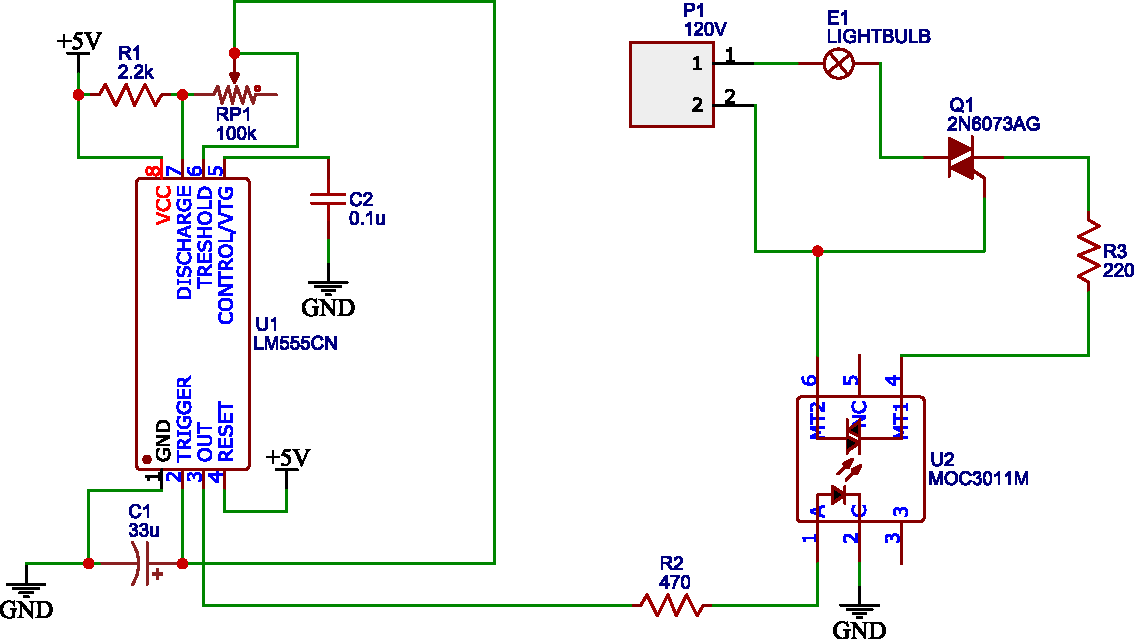
\includegraphics[width=0.8\textwidth]{media/circuito_09}
    \caption{Circuito utilizado en la práctica 9.}
    \label{Fig: Circuito utilizado en la practica 9}
\end{figure}

Como logramos obtener todos los componentes específicos que se pueden observar en la \cref{Fig: Circuito utilizado en la practica 9}, el circuito tanto téorico como práctico quedaron configurados y diseñados de la misma manera. Permitiéndonos aplicar las fórmulas presentadas con anterioridad.

\subsection{Resultados}

Al mover el potenciómetro, que es la resistencia $R_B$ en las fórmulas, hacia 0, el foco tiene un porcentaje del tiempo de encendido del 100\%, cumpliendo lo que debería de pasar. Por el otro lado, cuando el potenciómetro se lleva a su máximo valor, el porcentaje del tiempo de encendido es del 50\%, ya que el tiempo de encendido del LM555 no puede ser menor a esta magnitud. Esto quiere decir que el funcionamiento del circuito fue el correcto y se alineó a los resultados esperados con la teoría.

\subsection{Conclusiones}

Esta práctica nos ayudó a enteder y tener un poco de experiencia con el otro modo de funcionamiento de un LM555, ya que en las prácticas anteriores lo habíamos usado como un timer no reseteable, contrario a esta, en la que lo utilizamos como un generador de señal astable. esto nos ayudó a darnos cuenta de qué, gracias a la exactitud que provee este componente, esta configuración permite tener un gran control sobre los tiempo del ciclo de trabajo de salida, ya que, al utilizar la fórmula y obtener valores teóricos, los tiempos obtenidos en la práctica son, prácticamente, iguales, dando a relucir la exactitud y utilidad de este componente para sistemas que tengan que ver con tiempo.
